\documentclass[12pt]{article}
\usepackage[utf8]{inputenc}
\usepackage[T1]{fontenc}
\usepackage[polish]{babel}
\usepackage{geometry}
\usepackage{tabularx}
\usepackage[table,xcdraw]{xcolor}
\usepackage{color}
\usepackage{subfig}
\usepackage{sidecap}
\usepackage{wrapfig}
\usepackage{float}
\usepackage{enumerate}
\usepackage{graphicx}
\usepackage{multirow}
\setlength{\parindent}{24pt}
\usepackage{hyperref}
\usepackage{titlesec}
\titlelabel{\thetitle.\quad}
\usepackage{amsmath}
\usepackage{anyfontsize}
\usepackage{indentfirst}
\usepackage{listings}
\usepackage{multicol}
\usepackage{pgfplots}
\usepackage{fancyhdr}
\usepackage{units}

\usepackage[figurename=Grafika]{caption}

\pdfpageheight  297mm
\pdfpagewidth   210mm


\newgeometry{tmargin=1.8cm,bmargin=1.8cm,lmargin =1.8cm,rmargin=1.8cm}
\pagestyle{fancy}
\fancyhf{}
\rhead{\textit{Raport}}
\cfoot{ \thepage}
\lhead{\textit{Wizualizacja silosów zbożowych}}
\begin{document}
    \begin{titlepage}
\begin{figure}
	\centering
	\includegraphics[width=18cm]{//home/kubus/Obrazy/logo-Pwr.png}
	
	\label{fig:pwr}
\end{figure}
	\begin{center}
		\huge Wydział Elektroniki, Fotoniki i Mikrosystemów \\ 
		\vspace{40pt}
		\huge /* nazwa przedmiotu*/  \\
	\end{center}
	\vspace{60pt}
	\hrule
	\vspace{1pt}
	\hrule
	\begin{center}
		{\fontsize{40}{50}\selectfont /*numer sprawozdania*/\\ }
		\vspace{10pt}
		{\fontsize{25}{25}\selectfont /*tytuł sprawozdania  }
	\end{center}
	\hrule
	\vspace{1pt}
	\hrule
	\begin{flushright}
		\vspace{65pt}
		\textit{\Large Prowadzący:}\\
		
		\Large /*godność prowadzącego*/\\
		\vspace{10pt}
		\textit{\Large Wykonał:}\\
		
		\Large Jakub Kusz \\
	
	\end{flushright}
	\vspace{100pt}
	\begin{center}
		\large Wrocław, \today r.
	\end{center}
\end{titlepage}


    \tableofcontents
    \newpage
    \section{Charakterystyka tematu projektu} \label{ch: 1}
    Niniejszy projekt ma na celu stworzenie aplikacji służącej do wizualizacji silosów zbożowych. Aplikacja będzie wizualizować oraz 
    monitorować 3 kluczowe parametry dotyczące stanu silosów:
    \begin{itemize}
        \item wypełnienie,
        \item temperatura panująca wewnątrz,
        \item wilgotność panująca wewnątrz.
    \end{itemize} 
    Z perspektywy rolnika magazynującego zboże w silosach są to niezmiernie ważne informacje, dzięki nim będzie w stanie 
    w łatwy sposób szacować ilość zebranego plonu, monitorować wilgotność oraz temperaturę
    panującą w silosie, których zbyt wysokie wartości bardzo często są 
    wyznacznikiem tego, że w silosie rozpoczęły się procesy gnilne.
    \subsection{Główne cele aplikacji}
        Głównymi celami aplikacji będą:
        \begin{itemize}
            \item umożliwienie szybkiego i łatwego dostępu do informacji o stanie zboża w silosach,
            \item prezentowanie danych w przyjemniej i intuicyjnej formie graficznej,
            \item informowanie o zbliżaniu się do wartości krytycznych i przekroczeniu ich.
        \end{itemize}
    \subsection{Realizacja projektu}
            Aplikacja zostanie napisana w języku C++, wykorzystywać będzie bibliotekę Qt pozwalającą na tworzenie graficznego interfejsu użytkownika
            (GUI). Dane do wizualizacji udostępnianie będą przez zaprojektowany układ czujników, znajdujący się na makiecie silosów. 
    

   

    \section{Specyfikacja finalnego produktu}
    Finalnym efektem projektu będzie aplikacja pozwalająca na monitorowanie parametrów
    wymienionych w pkt. \ref{ch: 1} i system czujników zastępujący prawdziwe silosy zbożowe.
    \subsection{Aplikacja} 
        \subsubsection{Wymagania funkcjonalne}
            Wymagania funkcjonalne są to wymagania które określają działanie systemu i zaspokajają potrzeby użytkownika.
            Poniżej znajduje się lista wymagań funkcjonalnych, które finalna wersja aplikacji powinna spełniać:
            \begin{itemize}
                \item Możliwość przeglądu monitorowanych na bieżąco parametrów stanu silosów:
                \begin{itemize}
                    \item każdego z parametrów osobno,
                    \item wszystkich parametrów razem.
                \end{itemize}
                \item prowadzenie rejestru pomiarów,
                \item wizualizacja pomiarów historycznych z określonego okresu czasu,
                \item ostrzeganie o zbliżaniu się do wartości niebezpiecznych,
                \item alarmowanie po przekroczeniu wartości niebezpiecznych.
            \end{itemize}
        \subsubsection{Wymagania niefunkcjonalne}
        Wymagania niefunkcjonalne określają przede wszystkim oczekiwania co do samej jakości działania 
        aplikacji oraz pożądanego zachowania tworzonego systemu.Poniżej znajduje się lista wymagań 
        niefunkcjonalnych, które finalna wersja aplikacji powinna spełniać:

        \begin{itemize}
            \item Użyte technologie: 
            \begin{itemize}
                \item C++ 17,
                \item Qt 6,
            \end{itemize}
            \item możliwość zmiany rozmiaru ekranu i responsywność elementów GUI,
            \item wielojęzyczność,
            \item komunikacja z układem sensorów za pomocą portu szeregowego,
            \item przechowywanie danych historycznych w pliku CSV.
        \end{itemize}

    \subsection{System czujników}
        W celu realizowania odczytu z czujników zostanie skonstruowana prosta, niewielkich rozmiarów makieta silosów zbożowych, na której 
        zostaną osadzone odpowiednie czujniki:
        \begin{itemize}
            \item pomiary temperatury i wilgotności: DHT11,
            \item pomiar wypełniania: HC SR04.
        \end{itemize}
    
    
    \section{Terminarz realizacji poszczególnych podcelów}
    Lista podcelów z dokładnością do jednego tygodnia oraz wykres gantta (wykr. \ref{fig: gantt}):
\begin{itemize}
    \item 
        20.03.2023: Studia literatury 
    \item 
        27.03.2023: Projektowanie interfejsu graficznego
    \item 
        3.04.2023 : Projektowanie architektury systemu, projektowanie makiety i układu elektronicznego czujników
        \item PIERWSZY KAMIEŃ MILOWY: Ukończenie etapu projektowania
    \item 
        10.04.2023: Budowa makiety i układu elektronicznego czujników
    \item 
        17.04.2023: Testowanie działania układu elektronicznego czujników
    \item 
        24.04.2023: Implementacja głównych elementów GUI
    \item 
        1.05.2023: Implementacja głównych elementów GUI
    \item 
        8.05.2023: Testowanie głównych elementów GUI
    \item 
        15.05.2023: Implementacja komponentów logicznych aplikacji
    \item 
        22.05.2023: Testowanie komponentów logicznych aplikacji
    \item 
        29.05.2023: Implementacja pozostałych elementów GUI
    \item 
        5.06.2023: Testowanie pozostałych elementów GUI
    \item 
        12.06.2023: Integracja wszystkich komponentów, testowanie aplikacji
    \item 
        19.06.2023: Tworzenie raportu końcowego
    \item DRUGI KAMIEŃ MILOWY:  Złożenie raportu końcowego i prezentacja rezultatów
\end{itemize}

\begin{figure}
    \centering
    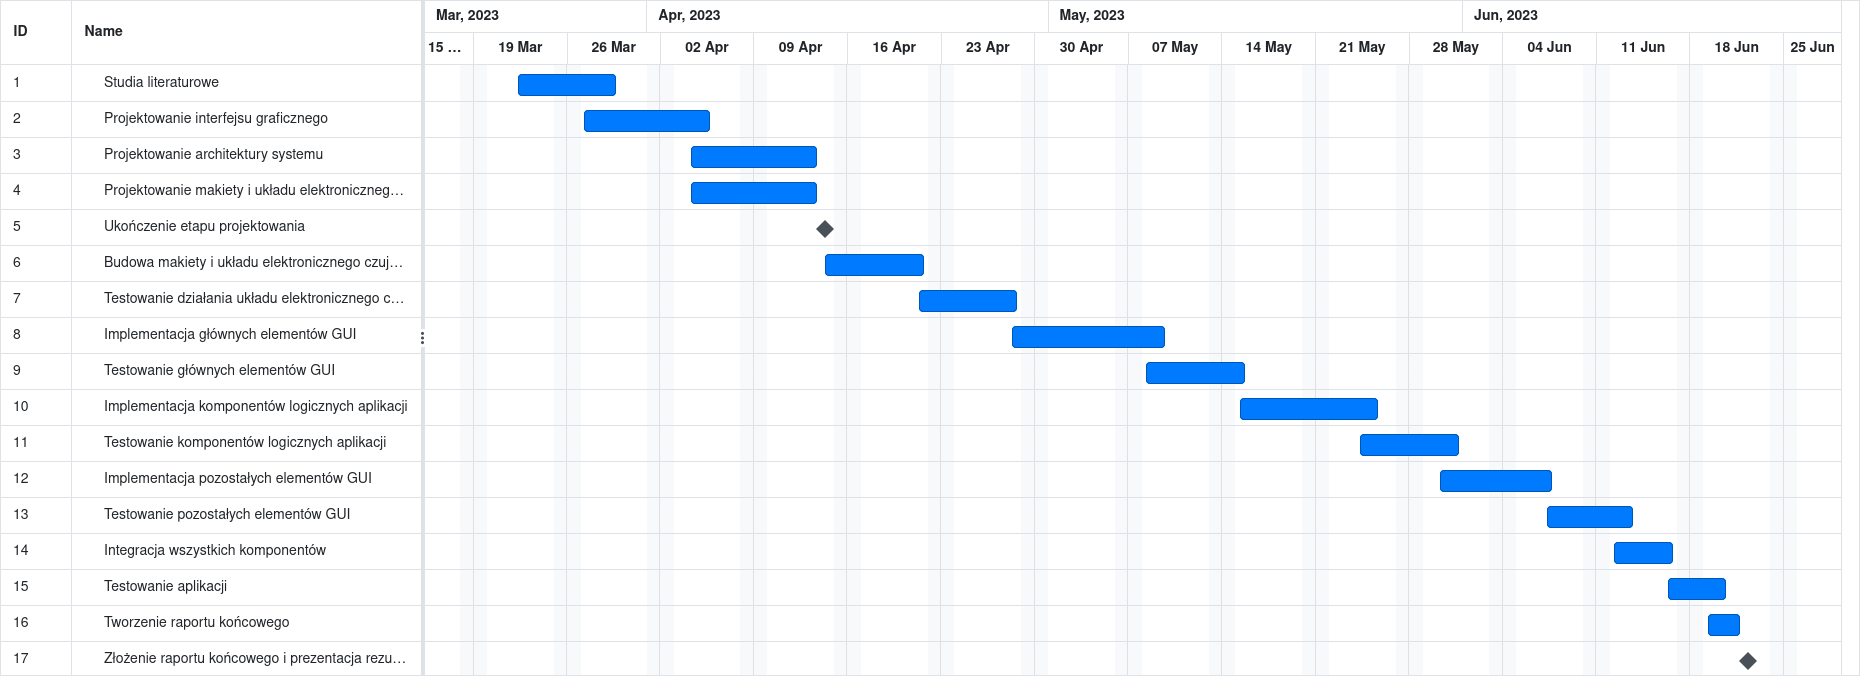
\includegraphics[width = \textheight, angle = 270]{obrazy/wsd_gantt.png}
    \caption{Wykres gantta}
    \label{fig: gantt}
\end{figure}

    \section{Projekt graficznego interfejsu użytkownika}
    Interfejs graficzny będzie przedstawiać w czterech wybieralnych zakładkach dwa silosy, na który prezentowane będą następujące elementy:
        \begin{itemize}
            \item widok wszystkich parametrów,
            \item widok wypełnienia,
            \item widok temperatury,
            \item widok wilgotności,
        \end{itemize}
    Ponadto dostępna będzie również piąta zakładka, prezentująca na wykresach dane historyczne.
    
    W kolejnych podpunktach zostaną przedstawione schematyczne grafiki prezentujące poszczególne widoki aplikacji
    na dane parametry.

    \subsection{Widok wszystkich parametrów}
        \begin{figure}[H]
            \centering
            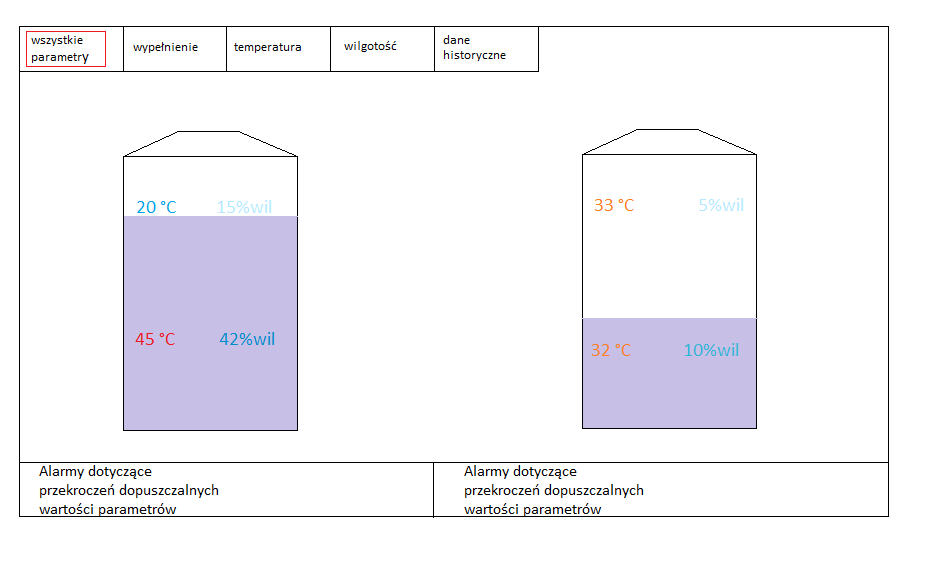
\includegraphics[width = \textwidth]{obrazy/projekt_grafiki/all.png}
            \caption{Widok na wszystkie parametry}
            \label{fig: all}
        \end{figure}
        Grafika \ref{fig: all} prezentuje idee poglądu na wszystkie parametry dotyczące silosów. Aby wybrać ten widok,
        w górnym pasku należy zaznaczyć opcje ,,wszystkie parametry''. Wypełnienie silosu symbolizowane jest kolorem. 
        w sposób tekstowy zaprezentowane zostaną wartości odczytane z czujników temperatury i wilgotności. Kolor czcionki
        będzie symbolizował wartość parametru, np. czerwony kolor czcionki będzie występował wraz ze wskazaniem temperatury 
        przekraczającej poziom alarmowy. Pod silosami znajdują sie pola przeznaczone do informowania o zaistniałych alarmach.
    \subsection{Widok wypełnienia}
        \begin{figure}[H]
            \centering
            \includegraphics[width = \textwidth]{obrazy/projekt_grafiki/wypełnienie.png}
            \caption{Widok na wypełnienie silosów}
            \label{fig: wypelnienie}
        \end{figure}

        Grafika \ref{fig: wypelnienie} prezentuje idee poglądu na wypełnienie silosów. Aby wybrać ten widok,
        w górnym pasku należy zaznaczyć opcje ,,wypełnienie''. Wypełnienie silosów symbolizowane będzie zapełnieniem
        obrysu silosów kolorem. Niski poziom będzie sygnalizowany na czerwono, poziomy bliskie połowy odcieniami żółtego,
        zbliżając się do maksymalnego poziomu kolor będzie stawał się zielony. Dodatkowo widoczna będzie informacja 
        o zapełnieniu silosów wyrażona w procentach.
    \subsection{Widok temperatury}
        \begin{figure}[H]
            \centering
            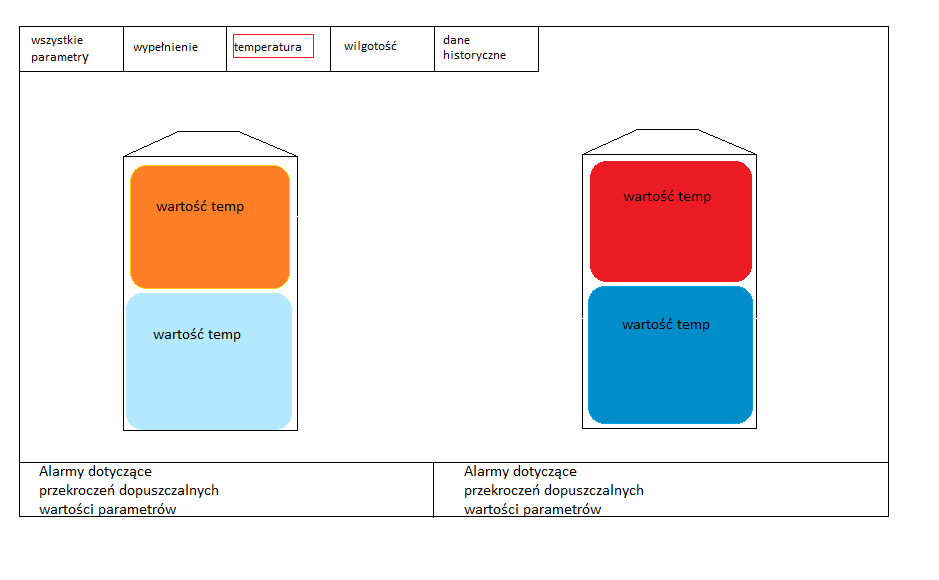
\includegraphics[width = \textwidth]{obrazy/projekt_grafiki/temperatura.png}
            \caption{Widok na temperature wewnątrz silosów}
            \label{fig: temperatura}
        \end{figure}

        Grafika \ref{fig: temperatura} prezentuje idee poglądu na temperature wewnątrz silosów. Aby wybrać ten widok,
        w górnym pasku należy zaznaczyć opcje ,,temperatura''. Temperatura symbolizowana będzie poprzez gradient kolorów,
        postały na podstawie odczytu temperatury z czujników. Odcienie niebieskiego będą symbolizować niskie temperatury,
        odcienie żółto-pomarańczowe średnie, a czerwone wysokie. Dodatkowo temperatura będzie prezentowana w formie 
        tekstowej.
    \subsection{Wilgotność}
        \begin{figure}[H]
            \centering
            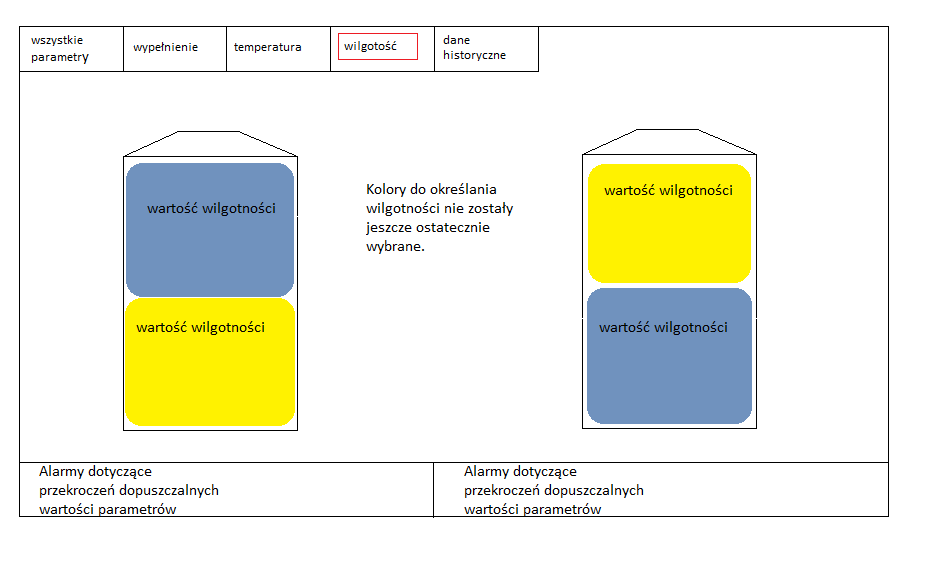
\includegraphics[width = \textwidth]{obrazy/projekt_grafiki/wilgotność.png}
            \caption{Widok na wilgotność wewnątrz silosów}
            \label{fig: wilgotnosc}
        \end{figure}
        Grafika \ref{fig: wilgotnosc} prezentuje idee poglądu na wilgotność wewnątrz silosów. Aby wybrać ten widok,
        w górnym pasku należy zaznaczyć opcje ,,wilgotność''. Wilgotność symbolizowana będzie poprzez gradient kolorów,
        postały na podstawie odczytu wilgotności z czujników. Nie ustalono jeszcze kolorystyki symbolizującej wilgotność, na grafice \ref{fig: wilgotnosc} kolory zostały wybrane przypadkowo. Dodatkowo wilgotność będzie prezentowana w formie 
        tekstowej.

    \subsection{Dane historyczne}
        \begin{figure}[H]
            \centering
            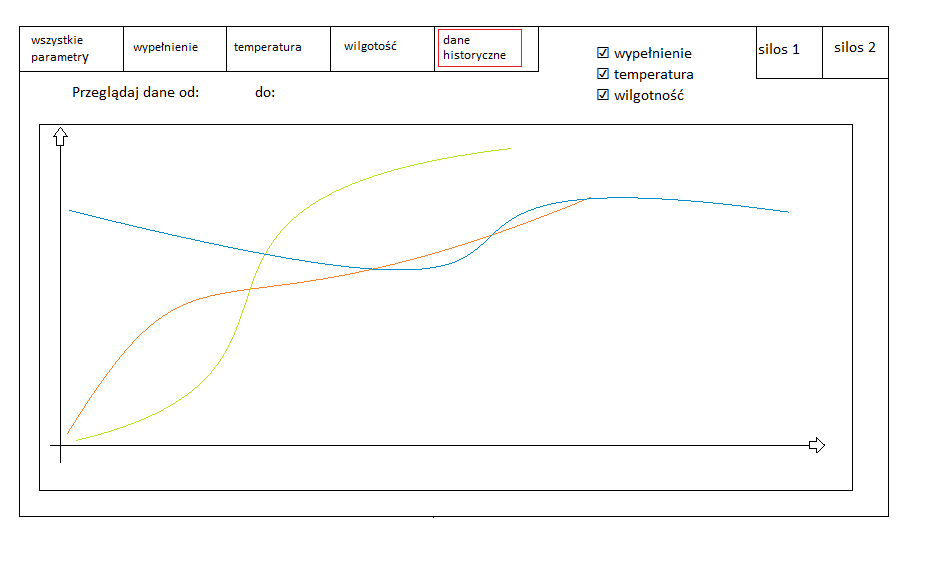
\includegraphics[width = \textwidth]{obrazy/projekt_grafiki/wykresy.png}
            \caption{Widok na dane historyczne}
            \label{fig: dane historyczne}
        \end{figure}
        Grafika \ref{fig: wilgotnosc} prezentuje idee poglądu na dane historyczne silosów. Aby wybrać ten widok,
        w górnym pasku należy zaznaczyć opcje ,,dane historyczne''. Widok ten przedstawia nam wykresy danych zapisanych i przechowanych przez aplikacje.
        Wykresy można poddać następującym modyfikacją:
        \begin{itemize}
            \item wybór silosu, którego dane chcemy wyświetlić,
            \item wybór danych, które mają zostać wyświetlone,
            \item wybór okresu czasu, z którego mają zostać zaprezentowane  dane.
        \end{itemize}
        
    \section{Prezentacja wyników pracy - 27.04.2023r.}
    Do dnia 27.04.2023r. wykonano następujące zadania:
    \begin{itemize}
        \item zaprojektowano układ czujników,
        \item opracowano transmisje danych z mikrokontrolera do komputera,
        \item określono sumę kontrolną dla opracowanej transmisji danych,
        \item zaprojektowano grafikę aplikacji,
        \item zaimplementowano zakładkę ,,wszystkie parametry''. 
    \end{itemize}

    \subsection{Protokół komunikacji}
        Komunikacja odbywa się poprzez UART. Ramka składa się z 13 bajtów. Dane 
        zbierane z czujników mogą okazać się większe niż 1 bajt wiec,
        przed wysłaniem dzielone są na 2 części i wysyłane jako 1 bajtowe. Program odbierający
        skleja je ze sobą do postaci 2 bajtowej. Dane wysyłane są w postaci  binarnej,
        w następujący sposób:
        \begin{itemize}
            \item Bajt 1: START -> 0xFF
            \item Bajt 2: OBJĘTOŚĆ -> 8 najstarszych bitów
            \item Bajt 3: OBJĘTOŚĆ -> 8 najmłodszych bitów
            \item Bajt 4: TEMPERATURA\_1 -> 8 najstarszych bitów
            \item Bajt 5: TEMPERATURA\_1 -> 8 najmłodszych  bitów
            \item Bajt 6: TEMPERATURA\_2 -> 8 najstarszych bitów
            \item Bajt 7: TEMPERATURA\_2 -> 8 najmłodszych  bitów
            \item Bajt 8: WILGOTNOŚĆ\_1 ->  8 najstarszych bitów
            \item Bajt 9: WILGOTNOŚĆ\_1 ->  8 najmłodszych bitów
            \item Bajt 10: WILGOTNOŚĆ\_2 ->  8 najstarszych  bitów
            \item Bajt 11: WILGOTNOŚĆ\_2 ->  8 najmłodszych  bitów
            \item Bajt 12: SUMA KONTROLNA -> CRC8
            \item Bajt 13: NUMER SILOSU -> 0xFE(silos 1) / 0xFD(silos 2)
        \end{itemize}
    \subsection{Aplikacja}
        \begin{figure}[H]
            \centering
            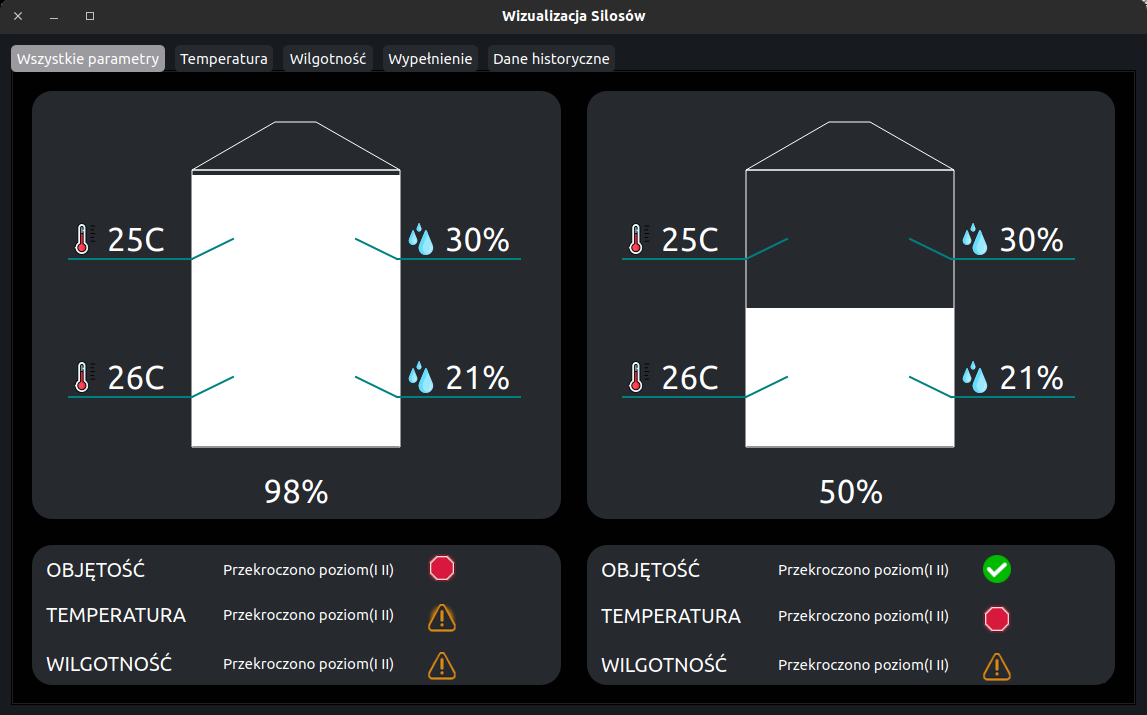
\includegraphics[width = \textwidth]{obrazy/zakladka_wszystkie_parametry.png}
            \caption{Wygląd zakładki wszystkie parametry}
        \end{figure}

        Ui zostało zaprojektowane za pomocą narzędzia Designer. Rysowanie silosów, ich wypełnienia i pozostałych 
        informacji zostało zrealizowane za pomocą reimplementacji metody painEvent. 
        Kod został udokumentowany za pomocą programu doxygen.
    \section{Prezentacja wyników pracy - 10.05.2023r}
    Do dnia 10.05.2023r. dokonano następujących postępów:
        \begin{itemize}
            \item zaimplementowano odczyt danych z portu szeregowego, poprzez uruchomienie go w osobnym wątku. 
                Obiekt będący kontenerem na dane przekazywany jest przez wskaźnik do obiektu \textit{main\_window}, dzięki
                czemu dane są dostępne dla pozostałych komponentów aplikacji.
            \item zaprojektowano interfejs widoku ,,Temperatura''.
            \item zaprojektowano interfejs okienka służącego ustawianiu wartości alarmów,
            \item połączono sloty odpowiedzialne za aktualizacje właściwych im danych dotyczących elementów interfejsu, takich jak:
                \begin{itemize}
                    \item graficzna i tekstowa  prezentacja wypełnienia silosu (widok ,,Wszystkie parametry''),
                    \item graficzna i tekstowa prezentacja temperatury (widoki ,,Wszystkie parametry'' i ,,Temperatura''),
                    \item Prezentacja informacji o alarmach  (widoki ,,Wszystkie parametry'' i ,,Temperatura''),
                \end{itemize}
            \item przebudowano strukturę aplikacji, odciążono obiekt \textit{main\_window}, w którym znajdowały się 
                wszystkie sloty wykorzystywane przez aplikację. Utworzono klasy ,,backendowe'' w których usystematyzowano
                kod dotyczący  slotów.
        \end{itemize}

\end{document}
